\documentclass{article}
\usepackage[paperheight=7in,paperwidth=7in, 
					top=0.5in, 
					bottom=0.5in, 
					left=0.5in, 
					right=0.5in]{geometry}
					
\usepackage[hidelinks]{hyperref}

\usepackage{tikz}
\usetikzlibrary{mindmap}

\begin{document}
\pagestyle{empty}

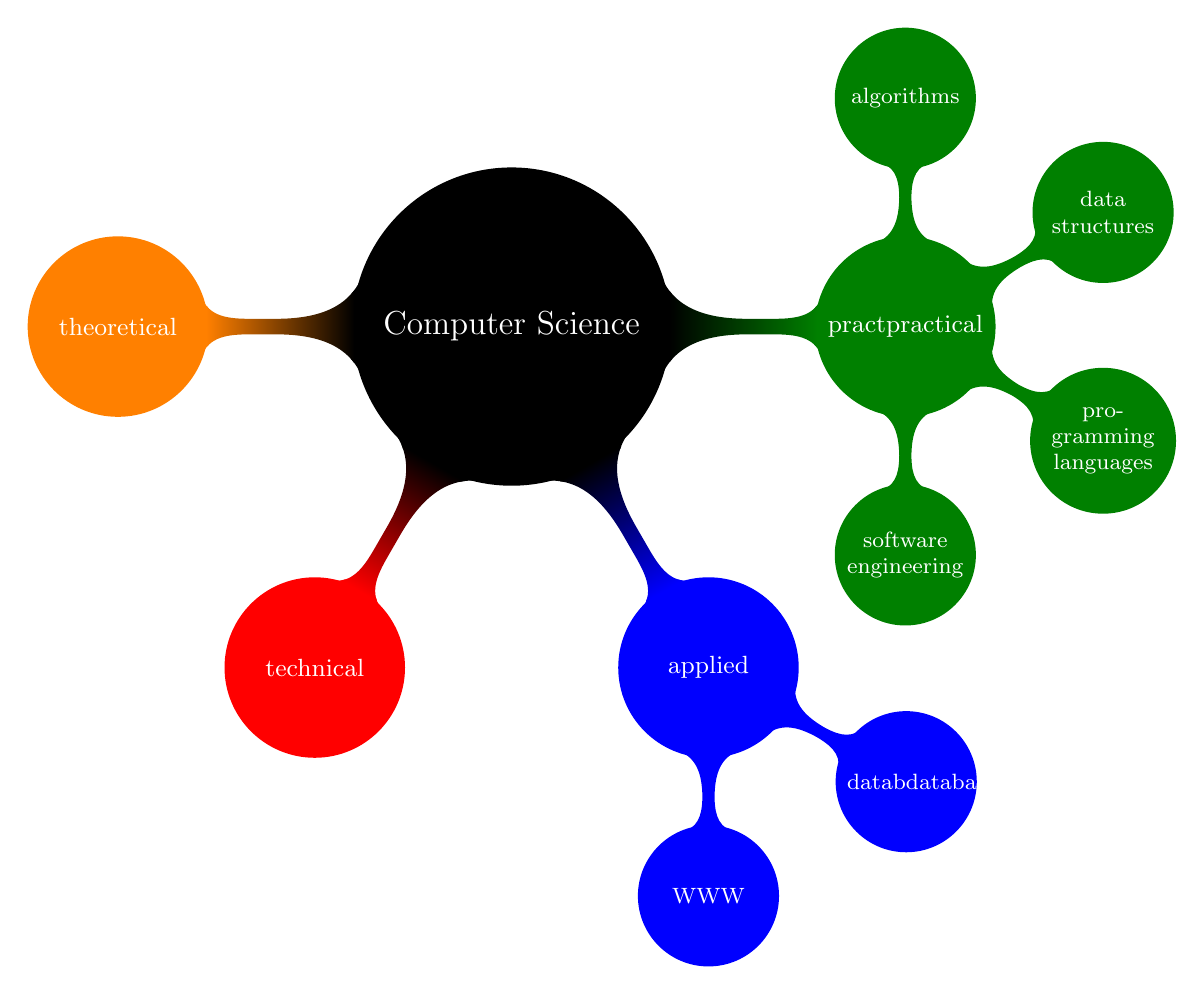
\begin{tikzpicture}
  \path[mindmap,concept color=black,text=white]
    node[concept] {Computer Science}
    [clockwise from=0]
    child[concept color=green!50!black] {
      node[concept] {\hyperlink{pract}{practical}}
      [clockwise from=90]
      child { node[concept] {algorithms} }
      child { node[concept] {data structures} }
      child { node[concept] {pro\-gramming languages} }
      child { node[concept] {software engineer\-ing} }
    }  
    child[concept color=blue] {
      node[concept] {applied}
      [clockwise from=-30]
      child { node[concept] {\hyperlink{datab}{databases}} }
      child { node[concept] {WWW} }
    }
    child[concept color=red] { node[concept] {technical} }
    child[concept color=orange] { node[concept] {theoretical} 
    };
\end{tikzpicture}
%\newpage
\begin{itemize}
\item \hypertarget{pract}{Practical}: here is some description.
\item \hypertarget{datab}{Databases}: here is some description.
\end{itemize}
\end{document}